

\tikzset{every picture/.style={line width=0.75pt}} %set default line width to 0.75pt

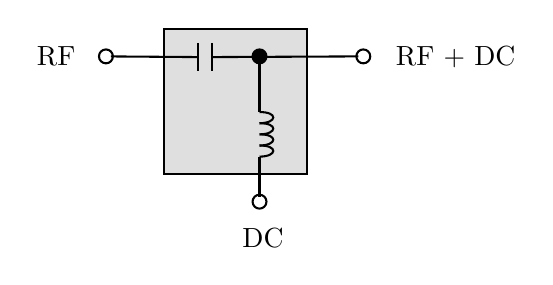
\begin{tikzpicture}[x=0.75pt,y=0.75pt,yscale=-1,xscale=1]
%uncomment if require: \path (0,300); %set diagram left start at 0, and has height of 300

%Shape: Rectangle [id:dp5847419531167373]
\draw  [fill={rgb, 255:red, 223; green, 223; blue, 223 }  ,fill opacity=1 ] (94,26.67) -- (162.67,26.67) -- (162.67,96.67) -- (94,96.67) -- cycle ;
%Straight Lines [id:da3655997692264292]
\draw    (68.35,40.02) -- (110.5,40.34) ;
\draw [shift={(66,40)}, rotate = 0.44] [color={rgb, 255:red, 0; green, 0; blue, 0 }  ][line width=0.75]      (0, 0) circle [x radius= 3.35, y radius= 3.35]   ;
%Straight Lines [id:da4762508902899607]
\draw    (117.13,40.34) -- (187.65,40.01) ;
\draw [shift={(190,40)}, rotate = 359.73] [color={rgb, 255:red, 0; green, 0; blue, 0 }  ][line width=0.75]      (0, 0) circle [x radius= 3.35, y radius= 3.35]   ;
%Straight Lines [id:da03465082932527963]
\draw    (110.5,33.51) -- (110.5,47.17) ;
%Straight Lines [id:da3348158883114294]
\draw    (117.13,33.51) -- (117.13,47.17) ;
%Straight Lines [id:da9848210218655242]
\draw    (140,40) -- (140,66.84) ;
\draw [shift={(140,40)}, rotate = 90] [color={rgb, 255:red, 0; green, 0; blue, 0 }  ][fill={rgb, 255:red, 0; green, 0; blue, 0 }  ][line width=0.75]      (0, 0) circle [x radius= 3.35, y radius= 3.35]   ;
%Straight Lines [id:da6955712196773951]
\draw    (140,88.31) -- (140,107.65) ;
\draw [shift={(140,110)}, rotate = 90] [color={rgb, 255:red, 0; green, 0; blue, 0 }  ][line width=0.75]      (0, 0) circle [x radius= 3.35, y radius= 3.35]   ;
%Curve Lines [id:da44310646563351463]
\draw    (140,66.84) .. controls (148.95,66.73) and (148.72,72.1) .. (140,72.21) ;
%Curve Lines [id:da7249179830921086]
\draw    (140,72.21) .. controls (148.95,72.1) and (148.72,77.47) .. (140,77.58) ;
%Curve Lines [id:da23791689791160175]
\draw    (140,77.58) .. controls (148.95,77.47) and (148.72,82.84) .. (140,82.95) ;
%Curve Lines [id:da12134770027518282]
\draw    (140,82.95) .. controls (148.95,82.84) and (148.72,88.21) .. (140,88.31) ;

% Text Node
\draw (42,39.83) node   [align=left] {RF};
% Text Node
\draw (234.5,40.5) node   [align=left] {RF + DC};
% Text Node
\draw (141.66,127.5) node   [align=left] {DC};


\end{tikzpicture}
